\section{Studies of the removal of CH$_3$T from LXe }
\label{sec:appendix1}

\newcommand*{\Scale}[2][4]{\scalebox{#1}{$#2$}}%

Prior to the first injection of CH$_3$T into LUX, we considered three risks that such a calibration may pose to the dark matter search: 1) that the xenon purification system may be ineffective for CH$_3$T removal; 2) that the interior surfaces of the stainless steel (SS)  gas handling system may become permanently contaminated with CH$_3$T; and 3) that the plastic detector components may outgas unacceptable quantities of CH$_3$T after initial exposure.

To address the first concern we studied the removal of natural methane (CH$_4$) from Xe gas with a heated Zr getter and a mass spectrometer. The purification efficiency was found to be satisfactory\cite{Dobi_CH4}. Furthermore, a test of the completed LUX purification system, including the actual getter unit, was performed several weeks before the first CH$_3$T injection into LUX. In this test $\sim$0.1 grams of CH$_4$ was injected into LUX, and mass spectrometry measurements of the CH$_4$ concentration in the LUX Xe gas were performed over the next several days. The CH$_4$ concentration was observed to decrease exponentially with a time constant of 5.90 $\pm 0.07$ hours as shown in Fig. \ref{fig:ch4_removal}, confirming the effectiveness of the purification system for methane removal.

The behavior of CH$_3$T in SS plumbing was studied in a bench-test with a custom-built Xe gas proportional tube operated at room temperature. Substantial quantities of CH$_3$T activity were injected, counted, and removed from the proportional tube. Initial tests found a small amount of residual activity after purification, however this was resolved by passing the CH$_3$T through a methane purifier (SAES model MC1-905F). No subsequent contamination was observed.

\begin{figure}[h!]
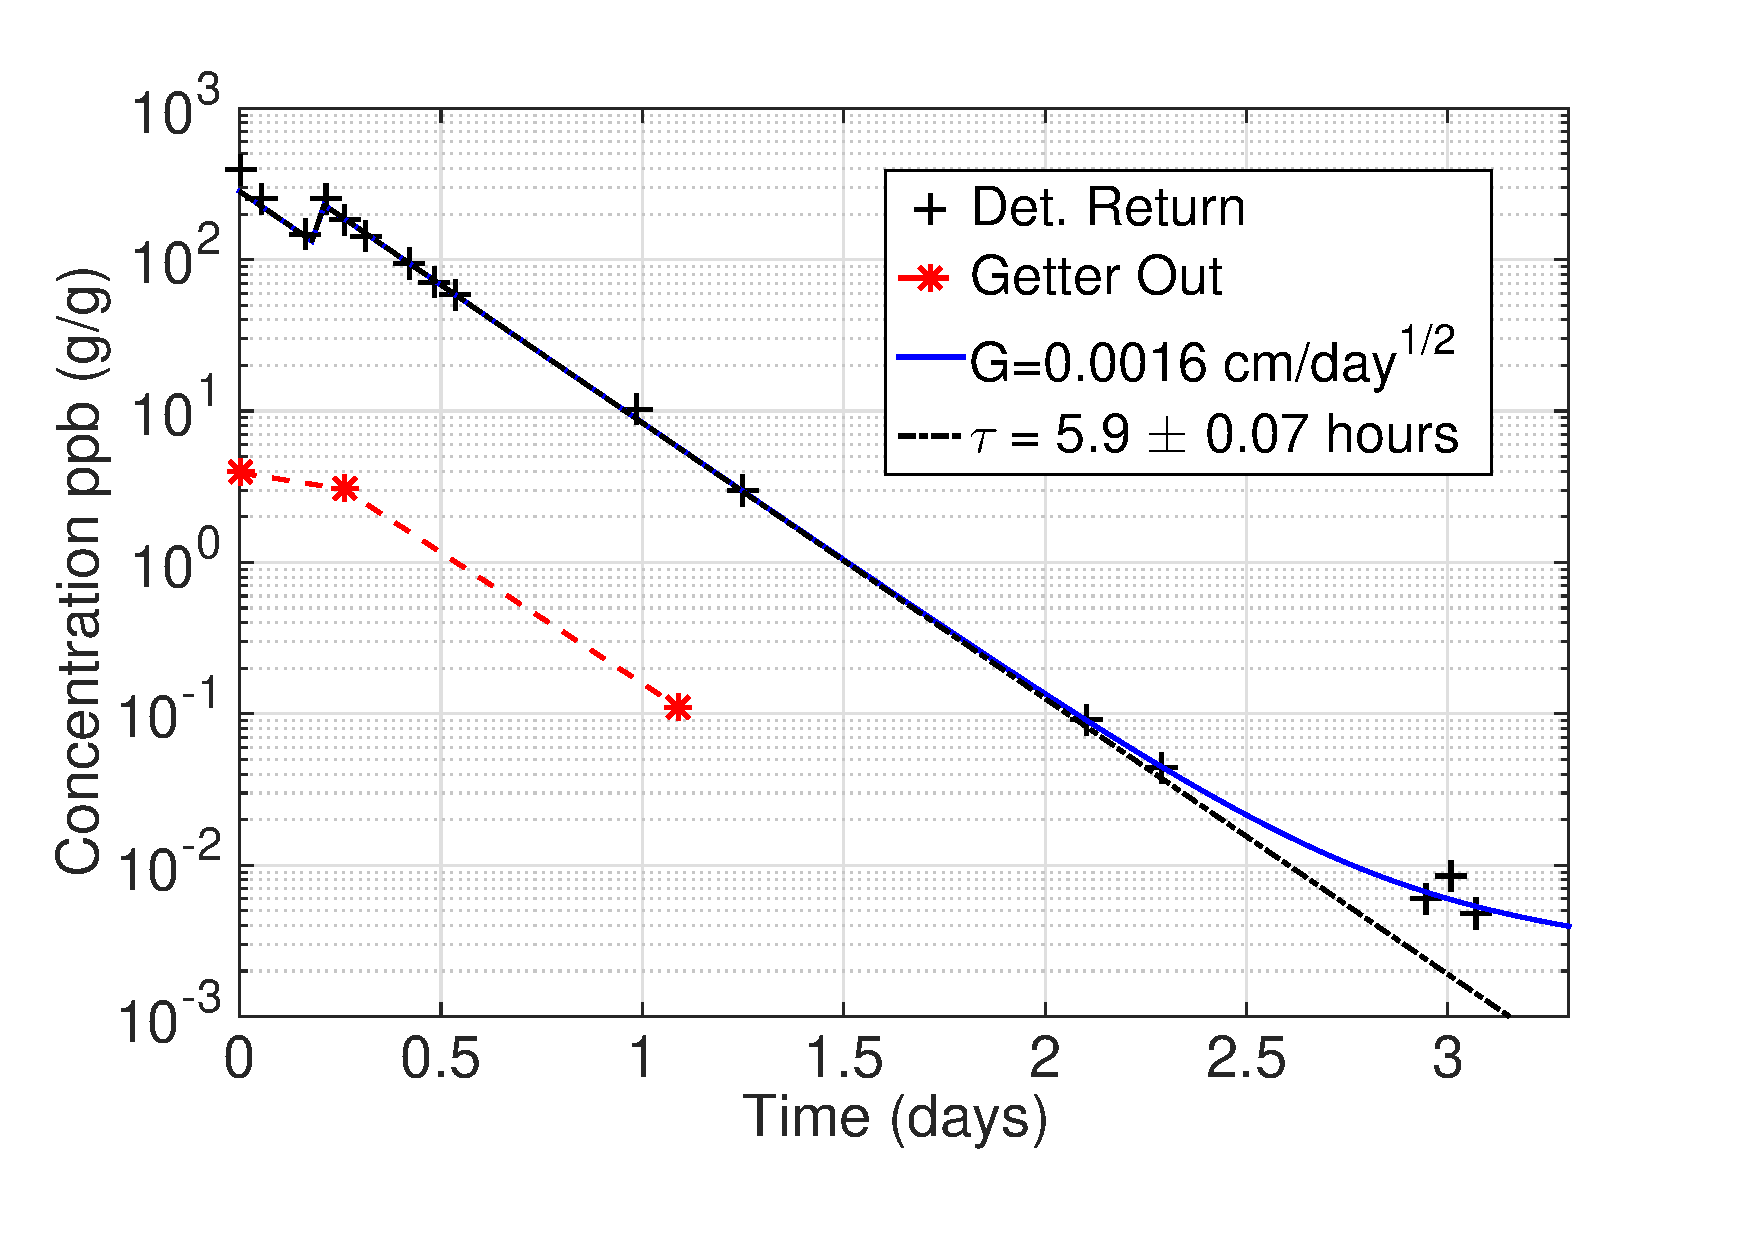
\includegraphics[width=80mm]{fig/July_CH4_wOG.eps}
\caption{Injection and removal of CH$_4$ in LUX prior to the first CH$_3$T injection. CH$_4$ is observed with a gas sampling mass spectrometry system. The black dashed lines shows an exponential fit to the CH$_4$ concentration at the detector return line with a time constant of 5.90 $\pm 0.07$ hours.  The red points indicate measurements at the getter outlet. We find a 97\% one-pass removal efficiency at a flow rate of 27 SLPM. The blue curve shows the upper limit on the effect of outgassing from the plastics. The three data points near t = 3 days are consistent with the limit of detection for methane ($\sim \rm 5\times10^{-3}$ ppb (g/g)) .}
\label{fig:ch4_removal}
\end{figure}

We also performed tests of CH$_3$T injection and removal from LXe with a small detector. One such experiment is shown in Fig. \ref{fig:Density}, where 68,000 Hz of CH$_3$T was injected, counted, and subsequently removed from LXe. Samples of LUX polyethylene and teflon were immersed in the LXe in this experiment, and their outgassing is evident in Fig. \ref{fig:Density}. These data placed constraints on the risk of CH$_3$T outgassing in LUX. In total over one million Hz of CH$_3$T activity was injected and successfully removed in these experiments.

\begin{figure}[h!]
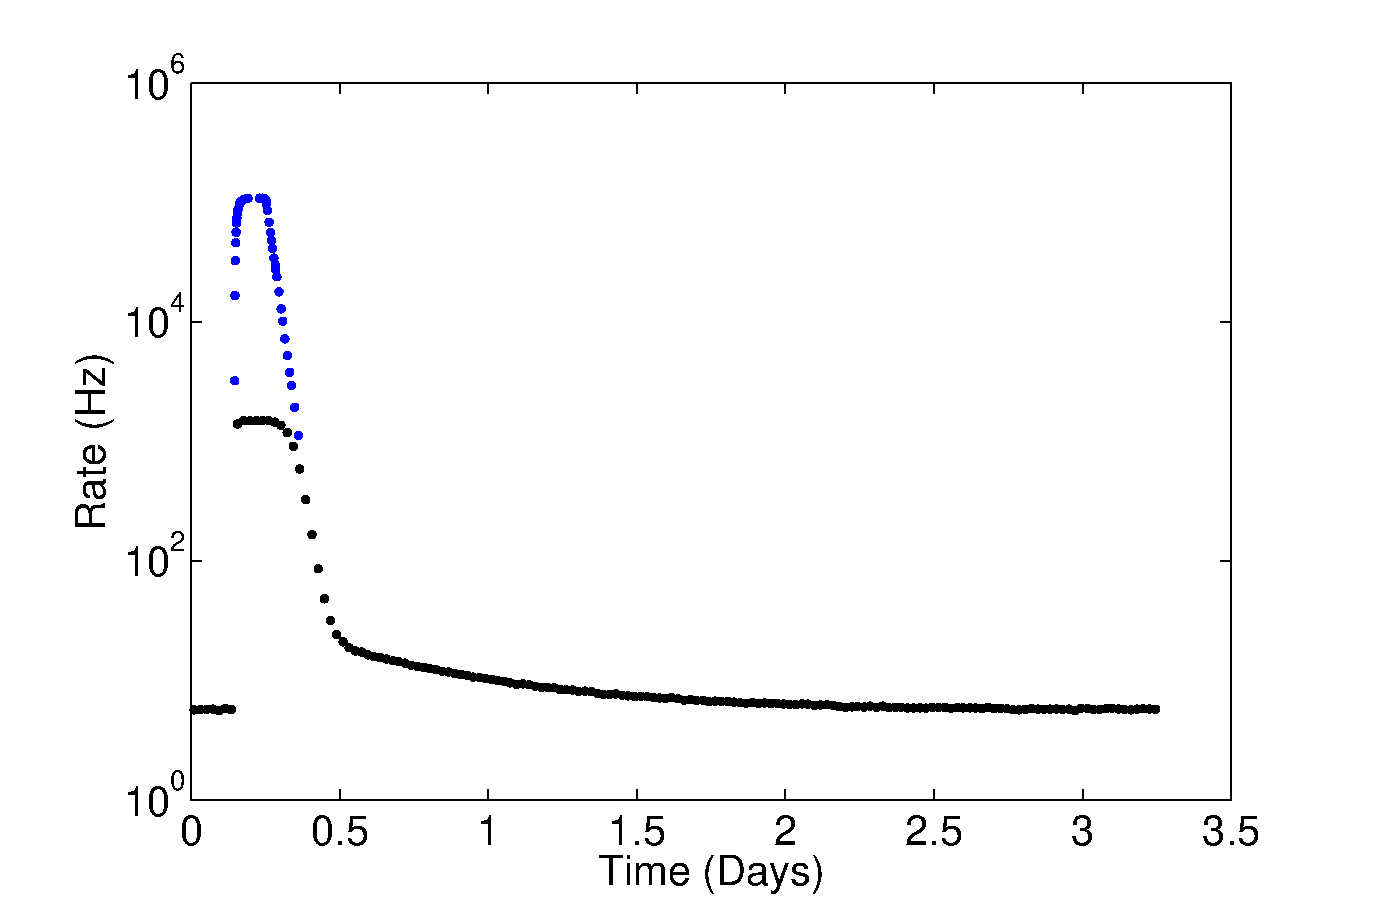
\includegraphics[width=80mm]{fig/TimeHisto_Analog2.eps}
\caption{The event rate versus time following a large CH$_3$T injection into a bench-top liquid xenon detector. Black points: the event rate measured with a dead-time limited digital DAQ system. Blue: true event rate measured with a fast analog scalar. In this experiment a maximum activity of 68,000 Hz was detected immediately after the injection, compared to a background count rate of 5 Hz. Initially the purifier is not included in the recirculation circuit, leading to a constant count rate. The count rate falls rapidly when the purifier is activated. At 0.5 days an elbow in the count rate is observed, indicating that outgassing of CH$_3$T from the detector plastics has become a limiting factor in the purification rate. }
\label{fig:Density}
\end{figure}


\section{Model of CH$_3$T removal}
\label{sec:appendix2}

We use a simple purification model to predict the CH$_3$T activity in LUX after an injection. The model is 

\begin{equation}
\frac{dC}{dt} = \frac{A}{V}J_{out} -\frac{C}{\tau},
\end{equation}

\noindent where  $C$ is the CH$_3$T concentration in the LXe,  $J_{out}$ is the flux of CH$_3$T out of the plastic components due to outgassing,  $A$ is the surface area of the plastic TPC cylinder, $V$ is the total volume of xenon in the active region, and $\tau$ is the characteristic removal time of CH$_3$T due to purification (5.9 hours). The model assumes perfect mixing of the fluid in the TPC. The initial concentration is the injection activity divided by the volume of the active region. We solve the model numerically with the Euler method while simultaneously solving the diffusion equation to determine $J_{out}$. The results predict the number of calibration events that may be collected and provide an estimate of when the CH$_3$T  decay rate will be small enough to allow the WIMP search to resume.

We approximate the diffusion into and out of the plastics as one-dimensional, since most plastics in LUX can be approximated as a thin cylindrical shell with no dependence on the azimuthal or $z$ coordinates.  Fick's laws in one dimension are

\begin{align}
J=-D\frac{d \phi(r,t)}{d r}  \\
\frac{d \phi}{d t} = D \frac{d^2 \phi(r,t)}{d r^2} 
\end{align}

\noindent 
where $J$ is the flux, $\phi(r,t)$ is the CH$_3$T  concentration in the plastic at depth $r$ and time $t$, and $D$ is the diffusion constant in the plastic. The concentration at the LXe-plastic boundary is fixed at $KC$, where K is the unitless solubility of CH$_3$T in the plastics. These equations are solved numerically and simultaneously with the purification model. 

$D$ and $K$ are not independently known for CH$_3$T in teflon or polyethylene at LXe temperature. However, only the combined quantity $G \equiv K \sqrt{ D/ \pi }$ is relevant as long as the diffusing substance does not reach the center of the plastic component (a good assumption for diffusion of CH$_3$T at LXe temperature). Under this condition, there exists an analytic solution to Fick's first law, which we evaluate at the LXe boundary:

%\begin{equation}
%\Scale[0.75]{\phi (x,t) = KC - \int \limits_0^t erf(\frac{x}{\sqrt{4D(t - \tau)}})K\frac{d}{d\tau}C(\tau)d\tau - KC(0)erf(\frac{x}{\sqrt{4Dt}}),}
%\end{equation}

\begin{equation}
J_{out}(t)= - G\left( \int \limits_0^t \frac{\frac{d}{dt'}C(t')}{\sqrt{t-t'}} dt' + \frac{C(0)}{\sqrt{t}}\right),
\end{equation}

\noindent
where the sign is reversed because the flux of material is outward. This result can be derived by applying Duhamel's principle along the infinite half-line, and it shows that the outgassing flux is linear in $G$. We set an upper limit of $G<0.0016 \frac{cm}{\sqrt{day}}$ for LUX based upon the data in Fig. \ref{fig:ch4_removal}. In that data the effect of $G$ would appear as an elbow in the CH$_4$ concentration versus time, as indicated by the blue line. The three data points near t = 3 days constrain the maximum value of $G$. We interpret this result as an upper limit because those data points are consistent with CH$_4$ backgrounds in the mass spectrometry system.

\begin{figure}[h!]
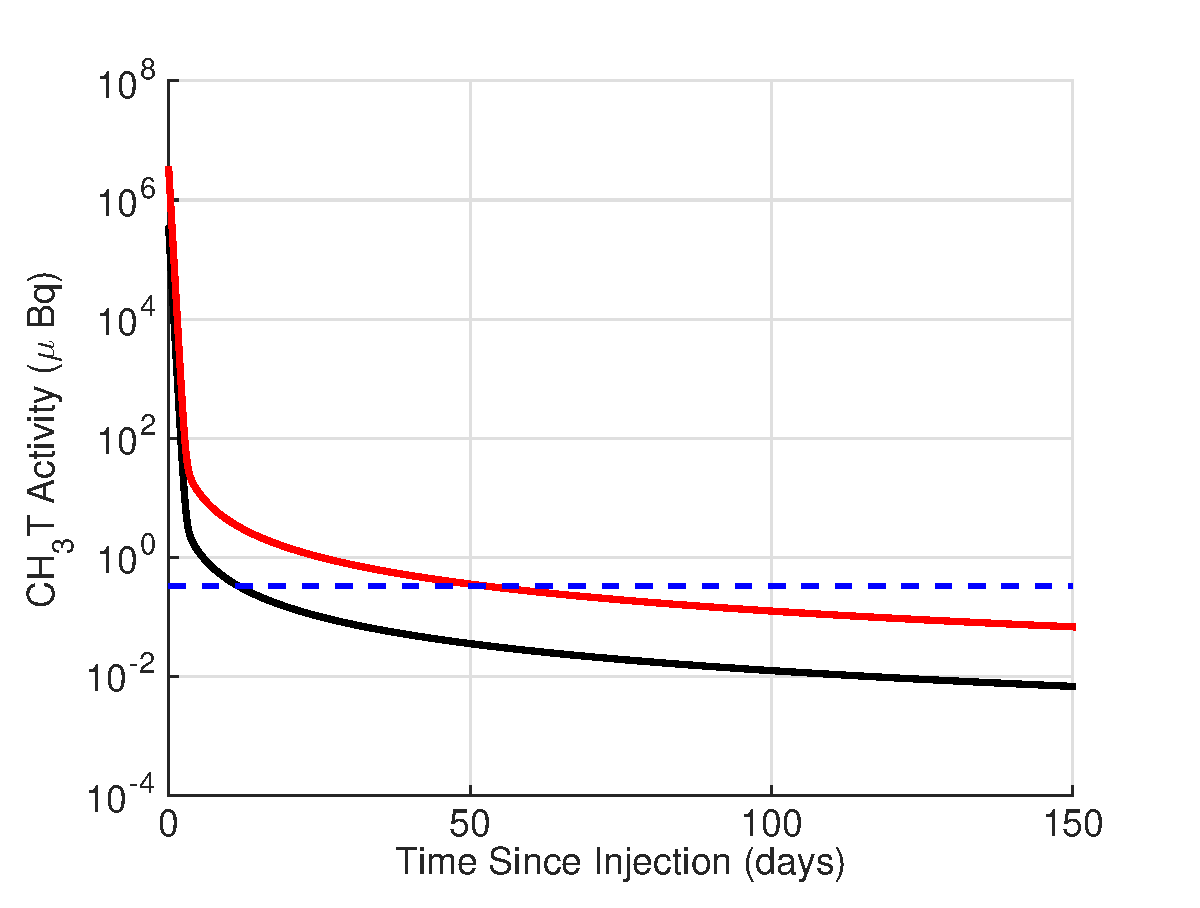
\includegraphics[width=0.95\textwidth]{fig/LUX_og_lim.eps}
\caption{Results of the purification model from 1 Bq (black curve) and 10 Bq (red curve) injections of CH$_3$T into LUX. The dashed blue line is the tritium activity goal of 0.33 $\mu$ Bq. The sharp initial fall is due to the 5.9 hour purification time constant of LUX, while the slow long-term removal is dominated by outgassing. The outgassing simulated here assumes  $G=0.0016$ cm/day$^{1/2}$).}
\label{fig:tau_var}
\end{figure}

Fig. \ref{fig:tau_var} shows the results of the purification model for a 1 Bq and 10 Bq injection into LUX assuming $G$ = 0.0016 cm/day$^{1/2}$  . We take 0.33 $\mu$Bq of residual CH$_3$T activity as an approximate goal for resuming WIMP search running, and we find that for injections on the order of 1 Bq we reach 0.33 $\mu$Bq eight days later, while 10 Bq injections may take as long as 35 days.  Ultimately the final decision regarding low background data quality is made during the data analysis phase, with guidance provided by the purification model described here.

\section{Light and charge yields of electron recoils in LXe at 180~V/cm and 105~V/cm}
\label{sec:appendix3}

Tables \ref{table:Yields} and \ref{table:Yields_100} list the light and charge yields of LXe for ER events between 1.3 and 17 keV and at fields of 180~V/cm and 105~V/cm, respectively. The uncertainties on the light and charge yields are highly anti-correlated in each energy bin due to the way in which the gain factors $g_1$ and $g_2$ are measured. The uncertainty listed includes both statistical and the dominant systematic uncertainty from the constraint on g1 and g2.

\begin{table}[h!]
\centering
\begin{tabular}{|c|c|c|c|} \hline
Energy 	& 		LY	& 	QY	& $\sigma$ \\ 
$\rm (keV_{ee}$) & ($\rm n_\gamma$/keV)   & ($\rm n_e$/keV) & ($\rm n$/keV) \\ \hline
1.3 	 & 14.6 	 & 58.4 	 & 2.2 	 \\ \hline 
1.5 	 & 17.3 	 & 55.7 	 & 1.9 	 \\ \hline 
2.0 	 & 22.3 	 & 50.7 	 & 2.4 	 \\ \hline 
2.5 	 & 27.4 	 & 45.6 	 & 2.5 	 \\ \hline 
3.0 	 & 31.5 	 & 41.4 	 & 2.3 	 \\ \hline 
3.5 	 & 33.8 	 & 39.2 	 & 2.0 	 \\ \hline 
4.0 	 & 35.8 	 & 37.2 	 & 2.2 	 \\ \hline 
4.5 	 & 37.5 	 & 35.5 	 & 2.0 	 \\ \hline 
5.0 	 & 38.4 	 & 34.6 	 & 1.9 	 \\ \hline 
5.2 	 & 38.9 	 & 34.1 	 & 2.0 	 \\ \hline 
5.5 	 & 39.5 	 & 33.5 	 & 2.1 	 \\ \hline 
6.0 	 & 40.4 	 & 32.6 	 & 2.0 	 \\ \hline 
6.5 	 & 41.7 	 & 31.3 	 & 2.0 	 \\ \hline 
7.0 	 & 41.7 	 & 31.3 	 & 1.7 	 \\ \hline 
7.5 	 & 42.7 	 & 30.3 	 & 2.0 	 \\ \hline 
8.0 	 & 42.9 	 & 30.1 	 & 1.9 	 \\ \hline 
9.0 	 & 43.8 	 & 29.1 	 & 1.7 	 \\ \hline 
10.0 	 & 44.7 	 & 28.3 	 & 2.0 	 \\ \hline 
11.0 	 & 45.4 	 & 27.6 	 & 1.7 	 \\ \hline 
12.0 	 & 46.0 	 & 27.0 	 & 1.7 	 \\ \hline 
13.0 	 & 46.5 	 & 26.5 	 & 1.5 	 \\ \hline 
14.0 	 & 47.1 	 & 25.9 	 & 1.6 	 \\ \hline 
16.0 	 & 46.4 	 & 26.6 	 & 2.5 	 \\ \hline 
17.0 	 & 44.9 	 & 28.1 	 & 2.5 	 \\ \hline 
\end{tabular}
\caption{Light and charge yield (photons/keV and electrons/keV) measured with tritium decay at 180~V/cm. The uncertainty includes both statistical and the dominant systematic uncertainty from the constraint on g1 and g2.}
\label{table:Yields}
\end{table}

\begin{table}[h!]
\centering
\begin{tabular}{|c|c|c|c|} \hline
Energy 	& 		LY	& 	QY	& $\sigma$ \\ 
$\rm (keV_{ee}$) & ($\rm n_\gamma$/keV)   & ($\rm n_e$/keV) & ($\rm n$/keV) \\ \hline
1.3 	 & 18.4 	 & 54.6 	 & 1.7 	 \\ \hline 
2.2 	 & 25.1 	 & 47.8 	 & 1.9 	 \\ \hline 
3.1 	 & 33.4 	 & 39.6 	 & 2.2 	 \\ \hline 
4.0 	 & 37.6 	 & 35.4 	 & 2.3 	 \\ \hline 
4.9 	 & 39.9 	 & 33.1 	 & 1.7 	 \\ \hline 
5.8 	 & 41.3 	 & 31.6 	 & 2.2 	 \\ \hline 
6.7 	 & 43.0 	 & 29.9 	 & 2.0 	 \\ \hline 
7.6 	 & 44.1 	 & 28.9 	 & 1.6 	 \\ \hline 
8.5 	 & 46.2 	 & 26.8 	 & 2.0 	 \\ \hline 
9.4 	 & 46.2 	 & 26.8 	 & 2.0 	 \\ \hline 
10.3 	 & 47.7 	 & 25.3 	 & 1.5 	 \\ \hline 
11.2 	 & 46.8 	 & 26.2 	 & 1.5 	 \\ \hline 
12.1 	 & 49.1 	 & 23.9 	 & 1.9 	 \\ \hline 
13.0 	 & 49.6 	 & 23.4 	 & 1.5 	 \\ \hline 
13.9 	 & 50.8 	 & 22.2 	 & 3.2 	 \\ \hline 
15.0 	 & 49.2 	 & 23.7 	 & 1.4 	 \\ \hline 
16.4 	 & 46.3 	 & 26.7 	 & 2.2 	 \\ \hline 
\end{tabular}
\caption{Light and charge yield (photons/keV and electrons/keV) measured with tritium decay at 105~V/cm. The uncertainty includes both statistical and the dominant systematic uncertainty from the constraint on g1 and g2. }
\label{table:Yields_100}
\end{table}


